\documentclass[notitlepage,a4paper]{article}

\usepackage{xltxtra}
\usepackage{amsmath}
\usepackage{tikz}
\usepackage{unicode-math}
\usepackage{fontspec}
\setmathfont{xits-math.otf}

\tikzset{node distance=2cm, auto}

\author{Víctor López Juan}
\title{Chapter 1}

\begin{document}

\maketitle

\begin{enumerate}
  \item[7.]
    
{\em Let $2 = \{a, b\}$ be any set with exactly 2 elements a and b. Define a functor
$F : Sets/2 → Sets × Sets$ with $F (f : X → 2) = (f^{−1} (a), f^{−1} (b))$. Is this
an isomorphism of categories?  }

    The category Sets/2 has:
    \begin{description}
      \item[Objects] The arrows (X → 2) in {\bf Set}
      \item[Arrows]  An arrow $\bar{f} : α : (A → 2) → β : (B → 2)$ for every
       function $f$ in {\bf Set} , $f : A → B$, such that the following diagram commutes:

        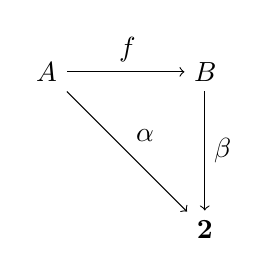
\begin{tikzpicture}
          \node (A) {$A$};
          \node (B) [right of=A] {$B$};
          \node (2) [below of=B] {$\text{\bf 2}$};
          \draw[->] (A) to node {$f$} (B);
          \draw[->] (A) to node {$α$} (2);
          \draw[->] (B) to node {$β$} (2);
        \end{tikzpicture}
    \end{description}

    The product category $\text{\bf C} × \text{\bf D}$, in general, entails:
    \begin{description}
      \item[Objects] Pairs of objects $(A,B)$, $A ∈ \text{\bf C}$, $B ∈ \text{\bf D}$.
      \item[Arrows]  $(f,g) : (A_1, B_1) → (A_2,B_2)$, where $f : A_1 → A_2$ and $g : B_1 → B₂$ arrows
        in $\text{\bf C}$, $\text{\bf D}$.
    \end{description}

    In particular, notice that, for every category $\text{\bf C}$, the product
    category $\text{\bf C} × \text{\bf C}$ can be constructed even if
    products are not defined in $\text{\bf C}$.
    
    The functor in the problem statement is defined as follows:
    
    \begin{equation*}
    \begin{array}{rll}
      F : & Sets/2           & → Sets × Sets              \\
          & α : (X → 2)      & → ( α^{-1}(a), α^{-1}(b) )      \\
          & \bar{f} : α → β  & → ( f|α^{-1}(a), f|α^{-1}(b) )  \\
    \end{array}
    \end{equation*}

    … where the symbol “$|$” means “restricted to”.

    Remember that, if $\bar{f} : α → β$, $α = β ◦ f$. This means that, for both $a,\,b ∈ \text{\bf 2}$:
    
    $$ x ∈ α^{-1}(a) \Leftrightarrow α(x) = a \Leftrightarrow (β \circ f)(x) = a \Leftrightarrow f(x) ∈ β^{-1}(a)$$
    $$ x ∈ α^{-1}(b) \Leftrightarrow α(x) = b \Leftrightarrow (β \circ f)(x) = b \Leftrightarrow f(x) ∈ β^{-1}(b)$$

    … therefore, $F(\bar{f}) : F(α) → F(β)$, so $F$ is well defined as a mapping.
    
    $F$ preserves identity and composition:

    $$F(id_{A→2}) = id_{(α^{-1}(a),α^{-1}(b))}$$

    And, if $\bar{g} : α → β$, $\bar{f} : β → γ$ …
    \begin{equation*}
    \begin{array}{rcl}
       & F(\bar{f} ◦ \bar{g})                        & = \\
    =  & ( (f ◦ g)|α^{-1}(a), (f ◦ g)|α^{-1}(b) )        & = \\
    =  & ( f|β^{-1}(a) ◦ g|α^{-1}(a), f|β^{-1}(b) ◦ g|α^{-1}(b) ) & = \\
    =  & ( f|β^{-1}(a) , f|β^{-1}(b) ) ◦ (g|α^{-1}(a) , g|α^{-1}(b) ) & = \\
    =  & F(\bar{f}) ◦ F(\bar{g}) & \\ 
    \end{array}
    \end{equation*}

    
    However, in order for $F$ to be an isomorphism, $F$ must be biyective
    on objects. This is not the case; as $F$ is not
    surjective.

    Suppose that $F$ is surjective, and a set $( \{1\}, \{1\} ) ∈ Set × Set$.

    Then, there is a set $A$, and $α : A → 2$, such that:

    $$F(α) = ( α^{-1}(a), α^{-1}(b) ) = ( \{1\}, \{1\} ) ∈ Set × Set$$

    This implies that $b = α(1) = a$, which is impossible. Therefore,
    $F$ is not biyective, nor an isomorphism.


    

   
{\em What about the analogous situation with a one element set 1 = {a} instead of 2?}

    Now:

    \begin{equation*}
    \begin{array}{rll}
      F : & Sets/1           & → Sets                   \\
          & α : (A → 1)      & → α^{-1}(a)   = A         \\
          & \bar{f} : α → β  & → f|α^{-1}(a) = f|A  = f  \\
    \end{array}
    \end{equation*}

    It is a functor, as it clearly respects identity and composition.

    \begin{itemize}
      \item {\bf 1} is a terminal object. Therefore, for every object X,
        including itself, there is a unique arrow $X → \text{\bf 1}$.
      \item For every arrow $f : A → B$ in Sets,the following diagram
        commutes:
        
  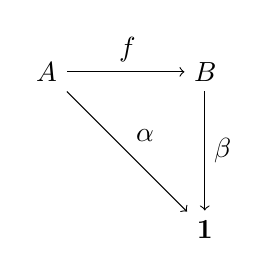
\begin{tikzpicture}
      
      \node (A) {$A$};
      \node (B) [right of=A] {$B$};
      \node (1) [below of=B] {$\text{\bf 1}$};
      \draw[->] (A) to node {$f$} (B);
      \draw[->] (A) to node {$α$} (1);
      \draw[->] (B) to node {$β$} (1);

  \end{tikzpicture}

     There's a unique arrow $α : A → 1$, so, if $f ◦ β : A → 1$,
     $f ◦ β = α$.

    \end{itemize}

    Therefore, the functor G is well defined:

    \begin{equation*}
    \begin{array}{rll}
      G : & Sets             & → Sets/1         \\
          & A                & α : A → 1  \\
          & f : A → B        & \bar{f} : α → β\\
    \end{array}
    \end{equation*}

    And is an inverse for F:

    $F ◦ G = G ◦ F = id$,

    which means that $F$ is an isomorphism, and $G$ is it's inverse
    
  \item[12.]

{\em
Verify the UMP for free categories on graphs, defined as above [the objects as
vertices], and arrows as sequences of edges. Specifically, let $C(G)$ be the free category on the
graph $G$, so defined, and $i : G → U (C(G))$ the graph homomorphism taking
vertices and edges to themselves, regarded as objects and arrows in $C(G)$.
Show that for any category {\bf D} and graph homomorphism $h : G → U (\text{\bf D})$,
there is a unique functor

$$\bar{h} : \text{\bf C}(G) → \text{\bf D}$$

with

 $$U(\bar{h}) ◦ i = h\text{ ,}$$
 
where $U : Cat → Graph$ is the underlying graph functor.

}

    We consider graphs as multigraphs, where parallel edges are allowed.

    The underlying graph functor can be defined as follows:

    \begin{equation*}
    \begin{array}{rll}
    U : & Cat         & → Graph            \\
        & (O, A)      & \mapsto (O, A, dom, cod) \\
        & F : C_1 → C_2 & \mapsto
            \begin{array}{rll}
              μ : & U(C_1)       & → U(C_2)                 \\
                  & v ∈ \text{vertices}(U(C_1))     & \mapsto F(v)                  \\
                  & e ∈ \text{edges}(U(C_1))       & \mapsto F(e) \\ 
            \end{array}
            \\
    \end{array}
    \end{equation*}

    To prove the UMP, we need to show existence and uniqueness of $\bar{h}$.
    
    \begin{description}
      \item[Existence]

        \begin{equation*}
          \begin{array}{rll}
            \bar{h} : & C(G)    & → D                                     \\
                      & \bar{h}(v)                & \mapsto  h(v)               \\                
                      & \bar{h}(id_v)             & \mapsto  id_{f(v)}            \\                
                      & \bar{h}(e_1 ◦ … ◦ e_n)    & \mapsto  h(e₁) ◦ … h(e_n)    \\                
          \end{array}
        \end{equation*}

        $\bar{h}$ satisfies $U(\bar{h}) ◦ i = h$ by construction. 

      \item[Uniqueness]

        
        Assume a functor $λ  : C(G) → D$ such that $U(λ) ◦ i = h$.

        Then, for every vertex $v$, it holds that:

          \begin{align*}
        λ(v) &= U(λ)(v)    \tag{definition of $U$} \\
             &= U(λ)(i(v)) \tag{definition of $i$} \\
             &= h(v)        \tag{hypothesis} \\
             &= \bar{h}(v)  \tag{definition of $\bar{h}$} \\
          \end{align*}
               

        And, $λ$ is a functor, so it must respect identity and composition:

        $$λ(id_V) = id_{λ(v)} = id_{h(v)} = \bar{h}(id_v)$$

          \begin{align*}
           λ(e_1 ◦ … ◦ e_n) &= λ(e_1) ◦ … ◦ λ(e_n)       \tag{$λ$ is a functor} \\
                            &= U(λ)(e_1) ◦ … ◦ U(λ)(e_n) \tag{definition of $U$} \\
                            &= h(e_1) ◦ … ◦ h(e_n)       \tag{hypothesis} \\
                            &= \bar{h}(e_1 ◦ … ◦ e_n)    \tag{definition of $\bar{h}$} \\  
          \end{align*}
    \end{description}

    Therefore, $\lambda = \bar{h}$.

\end{enumerate}


\end{document}
  
